\chapter{Manuel de jeu}
\section{Jouer une partie}
Lorsque vous rentrez en jeu, les joueurs et les balles sont placés à leur position initiale. Chaque type de joueur est identifié par une couleur: 
\textbf{bleu} pour les \gls{poursuiveur}s, \textbf{rouge} pour les \gls{batteur}s, \textbf{vert} pour le \gls{gardien} et \textbf{jaune} pour l' 
\gls{attrapeur}. 
Les joueurs aux costumes rayés sont ceux de votre adversaire, les vôtres sont en couleurs pleines.

\subsection{Sélection d'un joueur}
\begin{figure}[h!]
    \centering
    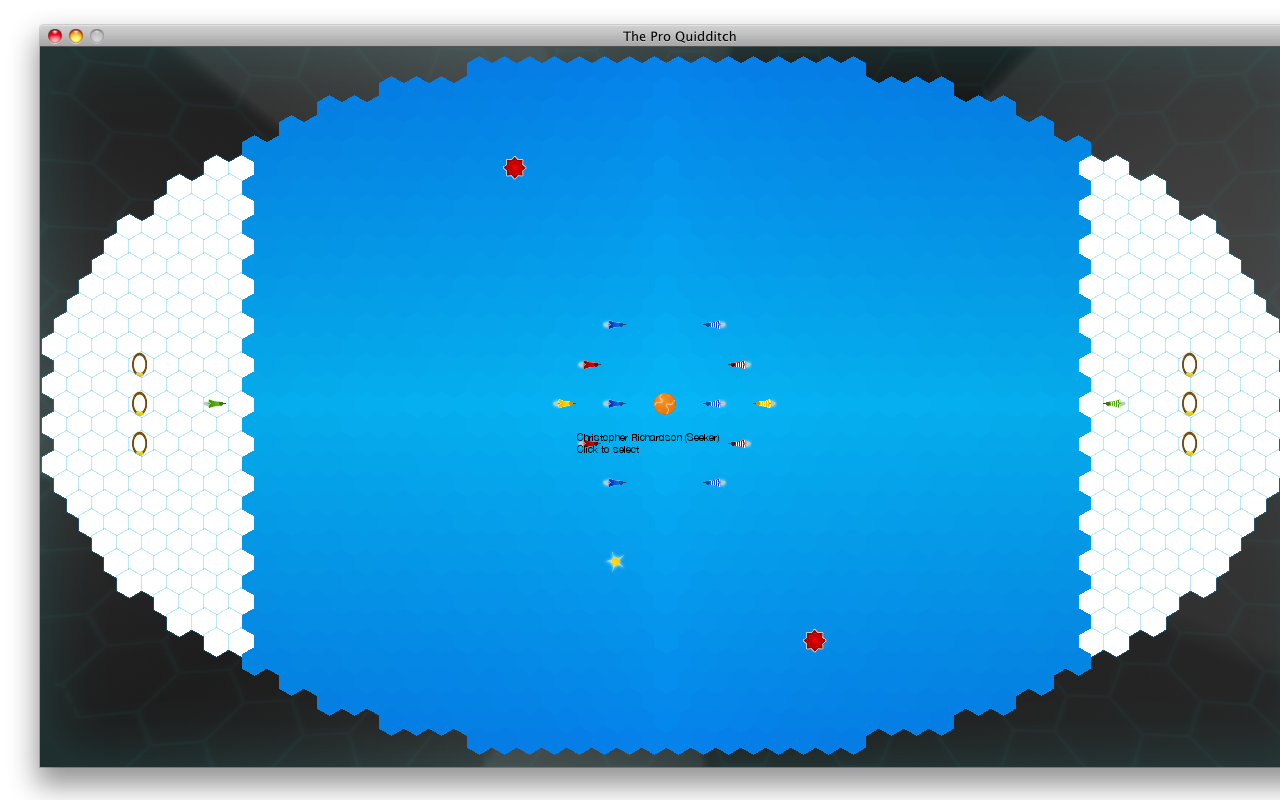
\includegraphics[width=\textwidth]{../screenshots/hover_seeker.png}
    \caption{\label{manual:view_name} Affichage du nom de l'attrapeur lorsque la souris le survole}
\end{figure}

Passez votre souris sur les joueurs pour découvrir leur nom (voir figure \ref{manual:view_name}). Comme l'outil d'aide le suggère, vous pouvez cliquer dessus pour les sélectionner. Une fois votre joueur sélectionné, les cases qu'il peut atteindre sont mises en évidence en jaune. Cliquez sur l'une d'elle: le chemin que parcourera votre joueur est affiché en rouge (voir figure \ref{manual:assign_move}). S'il peut encore continuer, les prochaines cases sont à nouveau mises en évidence en rouge. Pour terminer le mouvement d'un joueur, re-cliquez sur la dernière case atteinte. Le gardien doit toujours rester dans sa zone, et il est interdit de sortir du terrain.

\begin{figure}[h!]
    \centering
    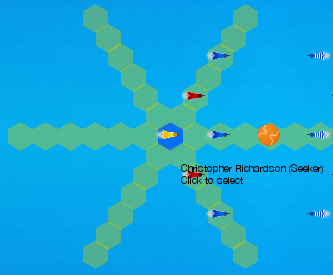
\includegraphics[width=0.45\textwidth]{../screenshots/assign_move.png}
    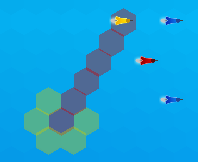
\includegraphics[width=0.45\textwidth]{../screenshots/assign_move2.png}
    \caption{\label{manual:assign_move} Affichage des cases atteignables par un joueur}
\end{figure}

\subsection{Actionner une balle}
Certains joueurs peuvent utiliser des balles. Les poursuiveurs peuvent attraper et lancer le \gls{souaffle}, et les batteurs peuvent taper les 
\gls{cognard}s. Lorsqu'une action de balle a lieu, le déplacement que l'on peut donner à la balle est indiqué en cases bleues.

\subsubsection{Souaffle}
Pour attraper le souaffle, il suffit qu'un poursuiveur ou un gardien passe sur la même case que lui. Quand un joueur est en possession du souaffle, il peut le lancer à toute case de son déplacement, en cliquant-droit sur la dernière position atteinte (indiquée en rouge). Les cases sur lesquelles il peut lancer la balle sont alors indiquées en bleu.

\begin{figure}[h!]
    \centering
    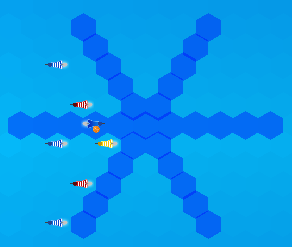
\includegraphics[width=0.5\textwidth]{../screenshots/throw_quaffle.png}
    \caption{\label{manual:throw_quaffle} Lancement du souaffle}
\end{figure}


\subsubsection{Cognards}
Pour lancer un cognard avec un batteur, il suffit de déplacer ce dernier sur la case de la balle. En cliquant sur la case de la balle, les marqueur bleus apparaîtront, vous permettant de battre la balle.

\begin{figure}[h!]
    \centering
    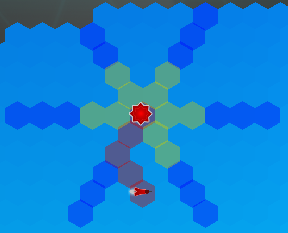
\includegraphics[width=0.5\textwidth]{../screenshots/throw_bludger.png}
    \caption{\label{manual:throw_bludger} Taper sur un cognard}
\end{figure}

\section{Gérer les installations}
Depuis le menu de gestion du stade, vous avez la possibilité d'acheter et d'améliorer trois types 
d'installations : des gradins, un fan shop et un stand de nourriture. Celles-ci vous rapporterons 
de l'argent à l'issue des matches en fonction de leur niveau et du nombre de téléspectateurs (lui
même dépendant de votre niveau réputation).

\begin{figure}[h!]
    \centering
    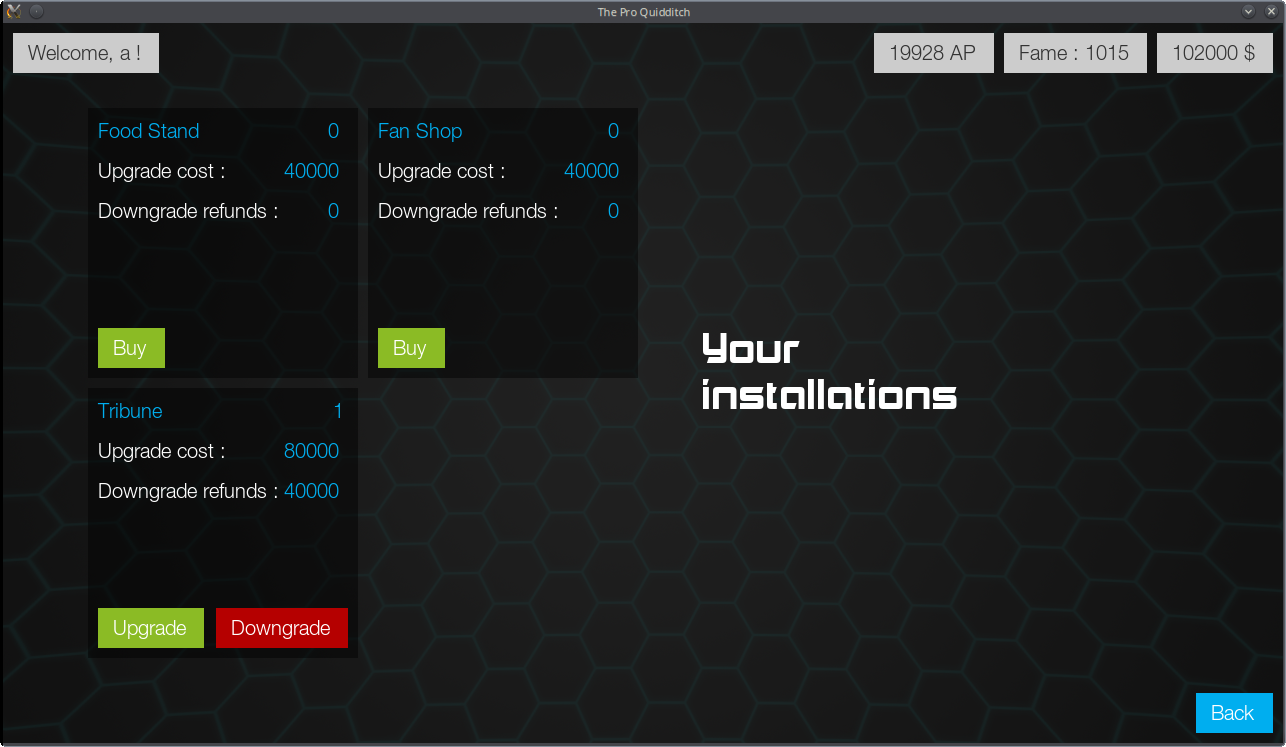
\includegraphics[width=0.5\textwidth]{../screenshots/installation_manager.png}
    \caption{\label{manual:installation} Menu de gestion des installations}
\end{figure}

\subsection{Acheter une installation}
Il faut pour cela, bien entendu, posséder les fonds suffisants.

Dans le jeu en interface graphique, il suffit de cliquer sur le bouton d'achat.

En ligne de commande, il s'agit de la première option (qui est confondue avec l'option d'amélioration.

\subsection{Améliorer une installation}
À nouveau, il faut disposer de suffisamment de fonds.

Dans le jeu en interface graphique, cliquez sur le bouton \emph{améliorer}.

En ligne de commande, il s'agit de la première option.

\subsection{Dégrader une installation}
Pour un manager tel que vous, trois choses sont absolument nécessaires : premièrement de l'argent,
ensuite de l'argent, et enfin de l'argent. Cependant, il vient un moment où celui-ci vient à nous 
manquer. Dégrader une installation permet de récupérer une partie des fonds dédiés à ses améliorations.

Dans le jeu en interface graphique, cliquez sur le bouton \emph{dégrader}.

En ligne de commande, il s'agit de la troisième option.

\section{Améliorer les caractéristiques des joueurs}
L'utilisateur peut augmenter l'efficacité de son équipe en améliorant le caractéristiques de ses joueurs. Ceci peut se faire de 2 manières : en ligne de commande et en interface graphique.
Les fonctionnalités sont analogues dans les 2 cas. Chaque "upgrade" coûte des points d'activité, le prix étant la valeur prochaine de la capacité du joueur. 
La valeur maximale d'une caractéristique ne peut pas dépasser  100.

